%%This is a very basic article template.
%%There is just one section and two subsections.
\documentclass{beamer}

\usepackage{calc,verbatim,amsmath,dsfont,subfig}
\usepackage{amsmath}
\newcommand{\given}{\mid}
\newcommand{\E}{\ensuremath{\mathds{E}}}

\usepackage{fontawesome}

\newcommand{\pros}{\item[\textcolor{green!80!black}\faThumbsUp]}
\newcommand{\cons}{\item[\textcolor{red!80!black}\faThumbsDown]}

% Setup appearance:

\usetheme{Frankfurt}

\usefonttheme[onlylarge]{structurebold}
\setbeamerfont*{frametitle}{size=\normalsize,series=\bfseries}
\setbeamertemplate{navigation symbols}{}

\definecolor{ubcblue}{RGB}{0,40,89}
\definecolor{ubcgray}{RGB}{116,145,163}

\setbeamercolor{section in toc}{fg=ubcblue,bg=white}
\setbeamercolor{alerted text}{fg=ubcblue}
\setbeamercolor*{palette primary}{fg=white,bg=ubcblue}
\setbeamercolor*{palette secondary}{fg=ubcblue,bg=ubcblue}
\setbeamercolor*{palette tertiary}{fg=white,bg=ubcblue}
\setbeamercolor*{palette quaternary}{fg=ubcgray!50!white,bg=ubcblue}

\setbeamercolor{item projected}{bg=ubcblue,fg=white}
\setbeamercolor{block title}{bg=ubcgray}
\setbeamercolor{block body}{bg=ubcgray!20!white}
\setbeamercolor{description item}{fg=ubcblue}
\setbeamercolor{caption name}{fg=ubcblue}

\setbeamerfont*{frametitle}{size=\Large}
\setbeamerfont*{title}{size=\Large}
\setbeamerfont*{section in toc}{size=\large}
\setbeamerfont*{block title}{}
\setbeamerfont*{item projected}{size=\footnotesize}
\setbeamerfont*{alerted text}{series=\bfseries}

\usepackage[english]{babel}
\usepackage[latin1]{inputenc}
\usepackage{animate}

\usepackage{times}
\renewcommand*\sfdefault{uop}

\usepackage[T1]{fontenc}

% Setup TikZ

\usepackage{tikz,pgfplots,siunitx,xfrac,comment,booktabs,etoolbox,multirow}
\robustify\bfseries
\newcommand{\minitab}[2][l]{\begin{tabular}{@{}#1@{}}#2\end{tabular}}

\sisetup{
  seperr,
  %repeatunits=false,
  product-units = single,
  trapambigerr=false,
  trapambigrange=false,
  %tophrase={{ bis }},
  valuemode=math,
  unitmode=math,
  quotient-mode=fraction,
  fraction-function=\sfrac
}

\usetikzlibrary{arrows,fadings,fit,positioning}
\usetikzlibrary{matrix,shadows}

\pgfdeclarelayer{background}
\pgfsetlayers{background,main}
%\pgfplotsset{every extra y tick/.append style={grid style=black}}
\usetikzlibrary{decorations,backgrounds,scopes,calc,decorations.pathreplacing}
\usetikzlibrary{shapes.geometric}

\newcounter{slidenumber}
\newcounter{pagesofcurrentframe}
\newlength{\slidenumberwidth}

\setbeamertemplate{footline}{
\setcounter{slidenumber}{\insertpagenumber}%
\addtocounter{slidenumber}{-\insertframestartpage}%
\addtocounter{slidenumber}{1}%
\setcounter{pagesofcurrentframe}{\insertframeendpage}
\addtocounter{pagesofcurrentframe}{-\insertframestartpage}
\addtocounter{pagesofcurrentframe}{1}
\normalfont 
\leavevmode
\hbox{
\begin{beamercolorbox}[wd=.98\paperwidth,ht=2.5ex,dp=2.125ex,leftskip=.3cm,rightskip=.3cm]{title in head/foot_}
\insertauthor
\hfill 
\insertshorttitle
\hfill
\settowidth{\slidenumberwidth}{\inserttotalframenumber}
\ifnum\value{pagesofcurrentframe}>1
\tikz[baseline=(char.base)] {
	\node[inner sep=0pt, text width=\slidenumberwidth,align=right] (char)
   	{\insertframenumber};
}%
\tikz[baseline=(char.base)] {
	\node[inner sep=0pt, text width=1em,align=left] (char)
   	{\alph{slidenumber}};
}
\else
\tikz[baseline=(char.base)] {
	\node[inner sep=0pt, text width=\slidenumberwidth,align=right] (char)
   	{\insertframenumber};
}%
\tikz[baseline=(char.base)] {
	\node[inner sep=0pt, text width=1em,align=left] (char)
   	{};
}
\fi
  \end{beamercolorbox}
}
}

\newcommand{\vect}[1]{\mathbf{#1}}

\newcommand{\watermarklogo}{
\includegraphics[width=4.5cm]{images/ubcblue.png}}

\usebackgroundtemplate{
\parbox[b][\paperheight+1.75cm]{\paperwidth+1cm}{
	\hfill\tikz 
	\node {\watermarklogo}
	node[fill=white,path fading=south,fading angle=45] {\phantom{\watermarklogo}}%
	node[fill=white,opacity=0.76] {\phantom{\watermarklogo}};
}
}

\newenvironment{questionmarks}{%
\usebackgroundtemplate{\parbox[b][%
\paperheight+1.45cm%
]{%
\paperwidth+1.45cm%
}{%
\hfill\tikz% 
\node {
\includegraphics[width=0.55\textwidth]{images/ubcquestions.png}}% 
node[fill=white,path fading=south,fading angle=45]%
{\phantom{
\includegraphics[width=0.55\textwidth]{images/ubcquestions.png}}}%
node[fill=white,opacity=0.3]%
{\phantom{
\includegraphics[width=0.55\textwidth]{images/ubcquestions.png}}}; }}%
}{%
\usebackgroundtemplate{%
\parbox[b][\paperheight+1.75cm]{\paperwidth+1cm}{%
	\hfill\tikz %
	\node {\watermarklogo}%
	node[fill=white,path fading=south,fading angle=45] {\phantom{\watermarklogo}}%
	node[fill=white,opacity=0.76] {\phantom{\watermarklogo}};%
}%
}%
}

\tikzstyle{simplenode}=[shape=circle,draw=black,
top color=ubcgray!5,bottom color=ubcgray!40,
semithick]
\tikzstyle{basicnode}=[simplenode,circular drop shadow]

\title[White Matter Lesion Segmentation by Deep Learning]{White Matter Lesion
Segmentation\\ by Deep Learning}

\author{Tom Brosch}

\institute[Universities of British Columbia]
{
MS/MRI Research Group\\
Electrical and Computer Engineering\\
The University of British Columbia
}

%\date{Ph.D. Proposal Defense}
\date{UBC MS Connect Presentation}

\begin{document}

\begin{frame}
\titlepage
\end{frame}

\makeatletter
\setbeamertemplate{enumerate items}{
    \llap{\begin{pgfpicture}{-1ex}{-0.8ex}{1ex}{1ex}
      {\pgftransformscale{0.9}\pgftext{\beamer@usesphere{section number
      projected}{tocsphere}}} \pgftext{%
        \usebeamerfont*{section number projected}%
        \usebeamercolor{section number projected}%
        \color{fg!90!bg}%
        \insertenumlabel}
    \end{pgfpicture}%
    %\kern0.15ex
    }%
}
\makeatother

\begin{frame}{Outline}
\tableofcontents
\end{frame}

\section{Introduction}

\subsection{Motivation}

\begin{frame}{Motivation}
\begin{itemize}
\item White matter lesions are a hallmark of MS
\item Imaging biomarkers for tracking disease progression and treatment effect,
e.g.:
\begin{itemize}
\item Lesion load
\item Lesion count
\end{itemize}
\item<2-> Lesions vary greatly in size, shape, intensity and location
\item<2->[$\Rightarrow$] \alert{Automatic and accurate segmentation
challenging!}
\end{itemize}
\uncover<2->{
\begin{center}
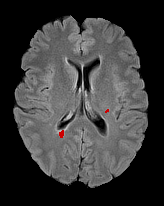
\includegraphics[height=0.3\textwidth]{images/fewlesions}\quad
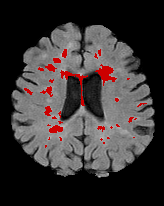
\includegraphics[height=0.3\textwidth]{images/manylesions}\quad
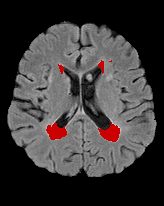
\includegraphics[height=0.3\textwidth]{images/periventricular}%
\end{center}
}
\end{frame}

\subsection{Related Work}

\begin{frame}{Related Work: Unsupervised methods}
\begin{description}
\item[Approach 1] 
Divide the intensities of brain MRIs into the four clusters
CSF, grey matter, white matter, and lesion voxels (e.g., lesion-TOADS)
\item[Approach 2] Model the intensity distribution of CSF, gray matter, and
white matter; lesions are outlines of that distribution (e.g., EMS)
\end{description}
\begin{itemize}
\pros<2-> Don't require labelled data for training
\pros<2-> Segmentation based on a per-subject per-image model
\pros<2-> Robust to inter-subject and inter-image variability
\cons<3-> Not specific to lesions
\cons<3-> Sensitive to non-lesion outliers such as blood vessels and partial
volume effects
\end{itemize}
\end{frame}

\begin{frame}{Related Work: Supervised methods}
\begin{description}
\item[Approach] Segmentation as a voxel classification problem
\item[Pipeline] Extract features $\Rightarrow$ classify voxel $\Rightarrow$
post-processing
\item[Features] Pre-defined or learned from unlabelled images
\item[Classifier] Random-forest, SVM, neural networks, library-based
\item[Post-processing] Markov random field, removal of isolated voxels
\end{description}
\begin{itemize}
\pros<2-> Lesion-specific
\cons<3-> Sensitive to inter-subject and inter-scanner variability
\cons<3-> Require large amounts of training data
\end{itemize}
\end{frame}

\begin{frame}{Related Work: End-to-end learning}
\begin{description}
\item[Main idea] Joint learning of features and classifier from labelled data
using a convolutional neural network (CNN)
\item[Approach 1] Classify image patches using a CNN (patch-based)
\item[Approach 2] Feed in entire volumes into a CNN\\ (fully convolutional)
\end{description}
\begin{itemize}
% \pros<2-> Lesion-specific
\pros<2-> Learning of features that are tuned to the data and segmentation
task
\pros<2-> Can learn features that are robust to inter-subject and inter-scanner
variability
\cons<3-> Requires large amounts of training data
\cons<3-> Training and inference of patch-based approaches can be prohibitively
slow
\end{itemize}
\end{frame}

\section{Method}

\subsection{Overview}

\begin{frame}{Method overview}
\begin{itemize}
\item Supervised method based on neural networks
\item Requires pairs of MRIs and corresponding segmentations
\item Learns parameters to perform segmentation
\end{itemize}
\end{frame}

\subsection{An Introduction to Neural Networks}

\begin{frame}{Neuron}
\begin{columns}[onlytextwidth]
\begin{column}{0.3\textwidth}
\centering
\footnotesize Nerve cell with synapse\\[0.5em]
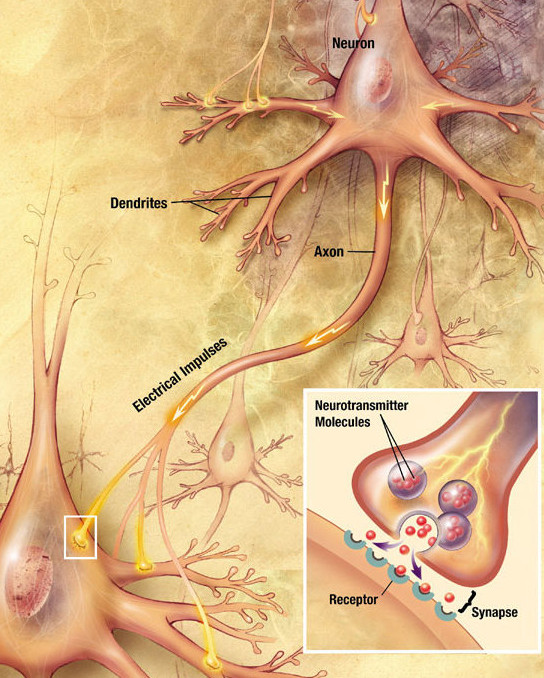
\includegraphics[width=\textwidth]{images/neuron1}
\end{column}
\begin{column}{0.45\textwidth}
\footnotesize \hspace{0.8em}Relationship between nerve cell\\\hspace{0.8em}and
neuron model:
\begin{itemize}
\item Neurotransmitters: inputs $x^{(0)}$ 
\item Excitatory/inhibitory receptor: weights $w^{(1)}$
\item Activation: weighted sum of its inputs
\item Action potential: output $x^{(1)}$
\end{itemize}
\end{column}
\begin{column}{0.25\textwidth}
\centering
\footnotesize Artificial neuron\\[0.5em]
\begin{tikzpicture}[scale=0.9]
\tikzstyle{neuron}=[draw,circle,minimum width=0.6cm]
\tikzstyle{every node}=[font=\small]
\tikzstyle{every label}=[align=center,font=\small]
\tikzstyle{every pin}=[align=center,font=\small]

\node[neuron,label=90:$x^{(1)}$] (output) at (2, 1.5) {};
\foreach \x in {0, 1, 2, 3} {
  \ifnum\x=3
    \node[neuron, label=90:$x^{(0)}_i$] (input\x) at (0, \x) {};
    
    \only<1> {
      \draw (input\x)--node[above=2pt] {$w^{(1)}_i$} (output);
    }
    \only<2> {
      \draw (input\x)--node[sloped,pos=0.4] {
        
\includegraphics[width=1.5em]{images/knob}} 
      (output);
    }
  \else
    \node[neuron] (input\x) at (0, \x) {};
    \only<1>{
      \draw (input\x)--node[above] {} (output);
    }
    \only<2> {
      \draw (input\x)--node[sloped,pos=0.4] {
        
\includegraphics[width=1.5em]{images/knob}}
      (output);
    }
  \fi
}
\end{tikzpicture}
\end{column}
\end{columns}
\begin{block}{Activation of a neuron}
\begin{equation*}
x^{(1)} = f\Big(\sum_i w^{(1)}_ix^{(0)}_i\Big)
\end{equation*}
\end{block}
\end{frame}

\begin{frame}{Fully Connected Neural Network}
\begin{center}
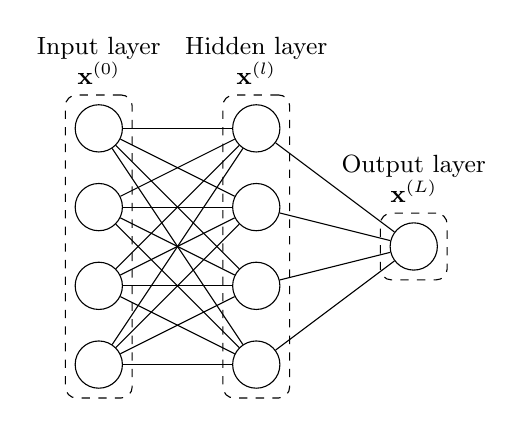
\begin{tikzpicture}

\tikzstyle{neuron}=[draw,circle,minimum width=0.6cm]
\tikzstyle{every node}=[font=\small]
\tikzstyle{every label}=[align=center,font=\small]

\foreach \x in {0, 1, 2, 3} {
  \node[neuron] (input\x) at (0, \x) {};
  \node[neuron] (hidden\x) at (2, \x) {};
}

\node[neuron] (output) at (4, 1.5) {};

\node[fit=(input0)(input3),draw,rounded corners=4pt, dashed,label=90:Input
layer\\$\vect{x}^{(0)}$] {};

\node[fit=(hidden0)(hidden3),draw,rounded corners=4pt, dashed,label=90:Hidden
layer\\$\vect{x}^{(l)}$] {};

\node[fit=(output),draw,rounded corners=4pt, dashed,label=90:Output
layer\\$\vect{x}^{(L)}$] {};

\foreach \x in {0, 1, 2, 3} {
  \foreach \y in {0, 1, 2, 3} {
    \draw (input\x)--(hidden\y);
  }
  \draw (hidden\x)--(output);
}
\end{tikzpicture}
\begin{block}{Activations of a layer of a neural network}
\vspace*{-1em}
\begin{align*}
\vect{x}^{(l)} &= f\big(\vect{W}^{(l)}\vect{x}^{(l-1)}\big) & \text{for }l \in
[1,L]
\end{align*}
\end{block}
\end{center}
\end{frame}


\begin{frame}{Reducing the Number of Weights}
\begin{columns}[onlytextwidth]
\begin{column}{0.45\textwidth}
%\centering
\begin{tikzpicture}

\tikzstyle{neuron}=[draw,circle,minimum width=0.6cm]
\tikzstyle{every node}=[font=\small]
\tikzstyle{every label}=[align=center,font=\small]

\foreach \x in {0, 1, 2, 3, 4} {
  \node[neuron] (input\x) at (0, \x) {};
}
\foreach \x in {1, 2, 3} {
  \node[neuron] (hidden\x) at (2, \x) {};
}

\node[neuron] (output) at (4, 2) {};

\node[fit=(input0)(input4),draw,rounded corners=4pt, dashed,label=90:$\vect{x}^{(0)}$] {};
\node[fit=(hidden1)(hidden3),draw,rounded corners=4pt, dashed,label=90:$\vect{x}^{(l)}$] {};
\node[fit=(output),draw,rounded corners=4pt, dashed,label=90:$\vect{x}^{(L)}$] {};

\only<1>{
  \foreach \x in {1, 2, 3} {
    \foreach \y in {0, 1, 2, 3, 4} {
      \draw (input\y)--(hidden\x);
    }
    \draw (hidden\x)--(output);
  }
}
\only<2>{
  \foreach \x in {1, 2, 3} {
    \draw (input\x)--(hidden\x);
    \pgfmathtruncatemacro{\layerindex}{\x-1}
    \draw (input\layerindex)--(hidden\x);
    \pgfmathtruncatemacro{\layerindex}{\x+1}
    \draw (input\layerindex)--(hidden\x);
    
    \draw (hidden\x)--(output);
  }
}
\only<3->{
  \foreach \x in {1, 2, 3} {
    \draw[green!80!black,thick] (input\x)--(hidden\x);
    
    \pgfmathtruncatemacro{\layerindex}{\x-1}
    \draw[blue!80!black,thick] (input\layerindex)--(hidden\x);
    
    \pgfmathtruncatemacro{\layerindex}{\x+1}
    \draw[red!80!black,thick] (input\layerindex)--(hidden\x);
    
    \draw (hidden\x)--(output);
  }
}
\end{tikzpicture}
\end{column}
\begin{column}{0.55\textwidth}
\begin{itemize}
\item<2-> Remove connections between distant neurons\\ (\alert{local
connectivity})
\item<3-> Use the same set of weights for neighboring neurons\\ (\alert{weight
sharing})
\item<3-> $\vect{W}=
\begin{pmatrix}
\textcolor{red!80!black}{k_1} & \textcolor{green!80!black}{k_2} &
\textcolor{blue!80!black}{k_3} & 0 & 0
\\
0 & \textcolor{red!80!black}{k_1} & \textcolor{green!80!black}{k_2} &
\textcolor{blue!80!black}{k_3} & 0 \\
0 & 0 & \textcolor{red!80!black}{k_1} & \textcolor{green!80!black}{k_2} &
\textcolor{blue!80!black}{k_3} \\
\end{pmatrix}$
\item<4-> $\vect{W}\vect{x} = \tilde{\vect{k}} * \vect{x}, \quad\vect{k} =
\begin{pmatrix} \textcolor{red!80!black}{k_1} & \textcolor{green!80!black}{k_2} &
\textcolor{blue!80!black}{k_3} \\
\end{pmatrix}$
\item<4->[$\Rightarrow$] \alert{Convolutional neural network}
\end{itemize}
\end{column}
\end{columns}
\end{frame}

\begin{frame}{Patch-based Convolutional Neural Networks}
\centering
\begin{tikzpicture}

\tikzstyle{neuron}=[draw,circle,minimum width=0.6cm]
\tikzstyle{every node}=[font=\small]
\tikzstyle{every label}=[align=center,font=\small]
\tikzstyle{every pin}=[align=center,font=\small,fill = white,overlay]

\only<1> {
\def\nodeindex{2}
\def\firstopacity{1}
\def\secondopacity{0}
}

\only<2-> {
\def\nodeindex{1}
\def\firstopacity{0.25}
\def\secondopacity{1}
}

\foreach \x in {-1, ..., 4} {
  \ifnum\x=\nodeindex
    \node[neuron,fill=ubcgray] (image\x) at (-1.5, \x) {};
  \else
    \node[neuron] (image\x) at (-1.5, \x) {};
  \fi
}

\node[fit=(image-1)(image4),draw,rounded corners=4pt,dashed,label=90:Image] {};

\begin{scope}[opacity=\firstopacity]

\foreach \x in {0, 1, 2, 3, 4} {
  \node[neuron] (input\x) at (0, \x) {};
}
\foreach \x in {1, 2, 3} {
  \node[neuron] (hidden\x) at (2, \x) {};
}

\node[neuron,fill=ubcgray] (output) at (4, 2) {};

\node[fit=(input0)(input4),draw,rounded corners=4pt, dashed,label=90:$\vect{x}^{(0)}$] {};
\node[fit=(hidden1)(hidden3),draw,rounded corners=4pt, dashed,label=90:$\vect{x}^{(l)}$] {};
\node[fit=(output),draw,rounded corners=4pt, dashed,label=90:$\vect{x}^{(L)}$] {};


\foreach \x in {1, 2, 3} {
  \draw (input\x)--(hidden\x);
  
  \pgfmathtruncatemacro{\layerindex}{\x-1}
  \draw (input\layerindex)--(hidden\x);
  
  \pgfmathtruncatemacro{\layerindex}{\x+1}
  \draw (input\layerindex)--(hidden\x);
  
  \draw (hidden\x)--(output);
}
\end{scope}

\begin{scope}[yshift=-1cm,opacity=\secondopacity]

\foreach \x in {0, 1, 2, 3, 4} {
  \node[neuron] (input\x) at (0, \x) {};
}
\foreach \x in {1, 2, 3} {
  \node[neuron] (hidden\x) at (2, \x) {};
}

\node[neuron,fill=ubcgray] (output) at (4, 2) {};

\node[fit=(input0)(input4),draw,rounded corners=4pt, dashed] {};
\node[fit=(hidden1)(hidden3),draw,rounded corners=4pt, dashed] {};
\node[fit=(output),draw,rounded corners=4pt, dashed] {};

\foreach \x in {1, 2, 3} {
  \draw (input\x)--(hidden\x);
  
  \pgfmathtruncatemacro{\layerindex}{\x-1}
  \draw (input\layerindex)--(hidden\x);
  
  \pgfmathtruncatemacro{\layerindex}{\x+1}
  \draw (input\layerindex)--(hidden\x);
  
  \draw (hidden\x)--(output);
}
\end{scope}

\node<3->[fit=(hidden2)(hidden3),ellipse,draw=red!80!black,thick,pin=80:Redundant\\
calculations] {};

\end{tikzpicture}
\end{frame}

\begin{frame}{Fully Convolutional Neural Networks}
\centering
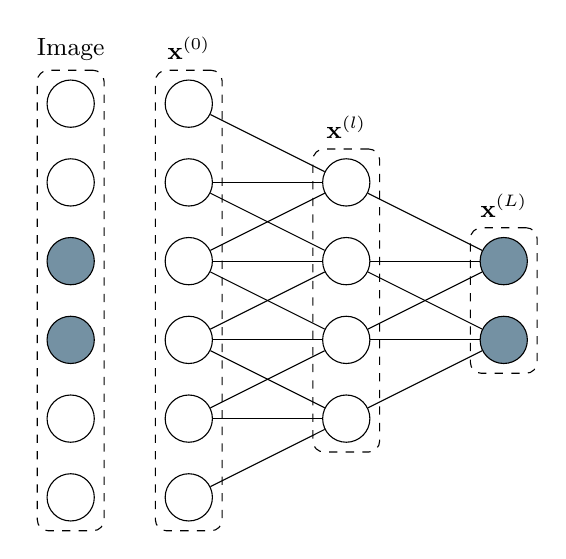
\begin{tikzpicture}

\tikzstyle{neuron}=[draw,circle,minimum width=0.6cm]
\tikzstyle{every node}=[font=\small]
\tikzstyle{every label}=[align=center,font=\small]
\tikzstyle{every pin}=[align=center,font=\small,fill = white,overlay]

\foreach \x in {-1, ..., 4} {
  \ifnum\x=2
    \node[neuron,fill=ubcgray] (image\x) at (-1.5, \x) {};
  \else
    \ifnum\x=1
      \node[neuron,fill=ubcgray] (image\x) at (-1.5, \x) {};
    \else
      \node[neuron] (image\x) at (-1.5, \x) {};
    \fi  
  \fi
}

\node[fit=(image-1)(image4),draw,rounded corners=4pt,dashed,label=90:Image] {};

\foreach \x in {-1, 0, 1, 2, 3, 4} {
  \node[neuron] (input\x) at (0, \x) {};
}
\foreach \x in {0, 1, 2, 3} {
  \node[neuron] (hidden\x) at (2, \x) {};
}

\foreach \x in {1, 2} {
  \node[neuron,fill=ubcgray] (output\x) at (4, \x) {};
}

\node[fit=(input-1)(input4),draw,rounded corners=4pt,
dashed,label=90:$\vect{x}^{(0)}$] {};
\node[fit=(hidden0)(hidden3),draw,rounded corners=4pt,
dashed,label=90:$\vect{x}^{(l)}$] {};
\node[fit=(output1)(output2),draw,rounded corners=4pt,
dashed,label=90:$\vect{x}^{(L)}$] {};

\foreach \x in {0, 1, 2, 3} {
  \draw (input\x)--(hidden\x);
  
  \pgfmathtruncatemacro{\layerindex}{\x-1}
  \draw (input\layerindex)--(hidden\x);
  
  \pgfmathtruncatemacro{\layerindex}{\x+1}
  \draw (input\layerindex)--(hidden\x);
}

\foreach \x in {1, 2} {
  \draw (hidden\x)--(output\x);
  
  \pgfmathtruncatemacro{\layerindex}{\x-1}
  \draw (hidden\layerindex)--(output\x);
  
  \pgfmathtruncatemacro{\layerindex}{\x+1}
  \draw (hidden\layerindex)--(output\x);
}

\end{tikzpicture}
\end{frame}

\begin{frame}{Convolutional Encoder Networks}
\centering
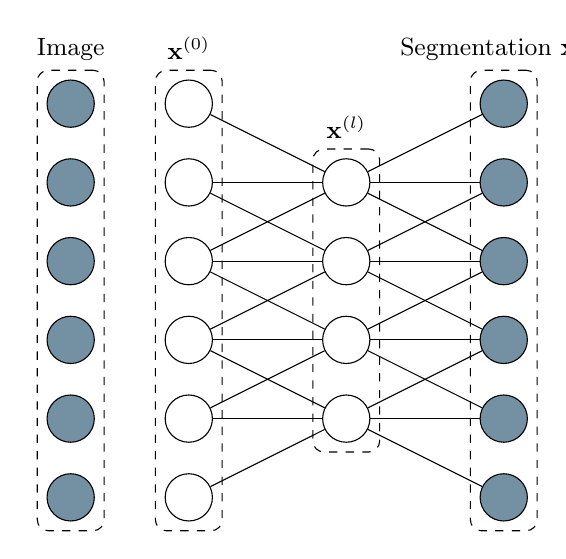
\begin{tikzpicture}

\tikzstyle{neuron}=[draw,circle,minimum width=0.6cm]
\tikzstyle{every node}=[font=\small]
\tikzstyle{every label}=[align=center,font=\small]
\tikzstyle{every pin}=[align=center,font=\small,fill = white,overlay]

\foreach \x in {-1, ..., 4} {
  \node[neuron,fill=ubcgray] (image\x) at (-1.5, \x) {};
}

\node[fit=(image-1)(image4),draw,rounded corners=4pt,dashed,label=90:Image] {};

\foreach \x in {-1, 0, 1, 2, 3, 4} {
  \node[neuron] (input\x) at (0, \x) {};
}
\foreach \x in {0, 1, 2, 3} {
  \node[neuron] (hidden\x) at (2, \x) {};
}

\foreach \x in {-1, 0, 1, 2, 3, 4} {
  \node[neuron,fill=ubcgray] (output\x) at (4, \x) {};
}

\node[fit=(input-1)(input4),draw,rounded corners=4pt,
dashed,label=90:$\vect{x}^{(0)}$] {};
\node[fit=(hidden0)(hidden3),draw,rounded corners=4pt,
dashed,label=90:$\vect{x}^{(l)}$] {};
\node[fit=(output-1)(output4),draw,rounded corners=4pt,
dashed,label={[overlay]90:Segmentation $\vect{x}^{(L)}$}] {};

\foreach \x in {0, 1, 2, 3} {
  \draw (input\x)--(hidden\x);
  \draw (output\x)--(hidden\x);
  
  \pgfmathtruncatemacro{\mylayerindex}{\x-1}
  \draw (input\mylayerindex)--(hidden\x);
  \draw (hidden\x)--(output\mylayerindex);
  
  \pgfmathtruncatemacro{\mylayerindex}{\x+1}
  \draw (input\mylayerindex)--(hidden\x);
  \draw (hidden\x)--(output\mylayerindex);
}

\end{tikzpicture}\\[0.5em]
\alert{Calculate segmentations of entire volumes in one forward pass!}
\end{frame}

\subsection{Network Architecture}

\begin{frame}[fragile]{Network Architecture: 3-layer CEN}
\begin{columns}
\begin{column}{0.45\textwidth}
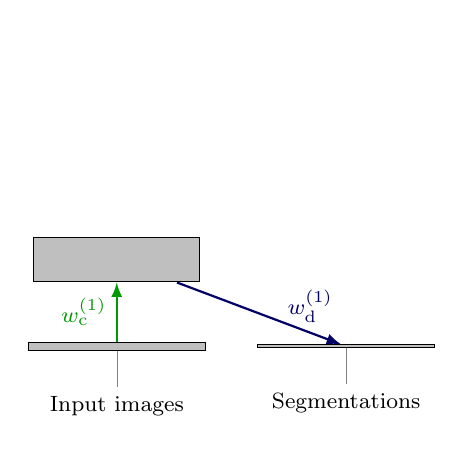
\begin{tikzpicture}[
  node distance=0.75cm and 0.65cm,
  font=\footnotesize,
  conv/.style={green!60!black,-latex,thick},
  conv2/.style={green!60!black,latex-latex,thick},
  deconv/.style={-latex,blue!40!black,thick},
  pooling/.style={-latex,green!60!black,thick,dashed},
  unpooling/.style={-latex,blue!40!black,thick,dashed},
  channel/.style args={#1 and #2}{draw, fill=lightgray, inner sep=0pt,
      minimum width=#1, minimum height=#2}
]

% Network

\node[channel=64pt and 3pt,pin=270:Input images] (inputs) {};
\node[channel=60pt and 16pt,above=of inputs] (clayer1) {};
\node[channel=64pt and 1pt,right=of inputs,pin=270:Segmentations] (outputs) {};

\begin{scope}[opacity=0]
\node[channel=30pt and 16pt,above=of clayer1] (pooling1) {};
\node[channel=60pt and 16pt] (dlayer1) at (clayer1-|outputs) {};
\node[channel=30pt and 16pt,above=of dlayer1] (dpooling1) {};
\node[fit=(pooling1)(dpooling1),inner sep = 0pt] (pooling) {};
\node[channel=26pt and 16pt,above=of pooling] (clayer2) {};
\end{scope}

\draw[conv] (inputs)--node[left] {$w^{(1)}_\text{c}$} (clayer1);
%\draw[pooling] (clayer1)--node[left] {} (pooling1);
%\draw[conv] (pooling1)--node[left] {$w^{(3)}_\text{c}$} (clayer2);
%\draw[deconv] (clayer2)--node[right=5pt] {$w^{(3)}_\text{d}$} (dpooling1);
%\draw[unpooling] (dpooling1)--node[right] {} (dlayer1);
%\draw[deconv] (dlayer1)--node[right] {$w^{(1)}_\text{d}$} (outputs);
\draw[deconv] (clayer1)--node[anchor=188,inner sep=10pt]
{$w^{(1)}_\text{d}$}(outputs);

\end{tikzpicture}
\end{column}
\begin{column}{0.55\textwidth}
\centering
\begin{tikzpicture}
\node[inner sep=0pt] (image) {
  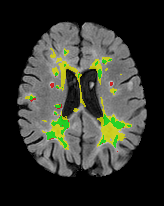
\includegraphics[width=0.45\textwidth]{images/p50s35_large_lesions_a}
};
\draw[white,thick] (-11pt,-14pt) circle (8pt);
\draw[white,thick] (13pt,-14pt) circle (9pt);

\end{tikzpicture}%
\hspace{4pt}%
\begin{tikzpicture}
[spy using outlines={circle, magnification=4, connect spies}]

\node[inner sep=0pt] (image) {
  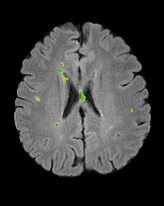
\includegraphics[width=0.45\textwidth]{images/p25s35_small_lesions_a}
};
\spy[white,thick, size=24pt,magnification=8] on (-9pt,18pt) in node[overlay]
at (-20pt,44pt);
\spy[white,thick, size=40pt] on (0pt,3pt) in node[overlay] at (24pt, 44pt);
\spy[white,thick, size=24pt, magnification=6] on (-11.5pt,-10.5pt) in
node[overlay] at (10pt,-46pt);

\node[below=1.5em of image,overlay,font=\footnotesize,align=right] {%
\textcolor{green!80!black}{Detected lesions}\\
\textcolor{yellow!80!black}{Missed lesions}\\
\textcolor{red!80!black}{False positives}};
\end{tikzpicture}
\end{column}
\end{columns}
\end{frame}

\begin{frame}[fragile]{Network Architecture: 7-layer CEN}
\begin{columns}
\begin{column}{0.45\textwidth}
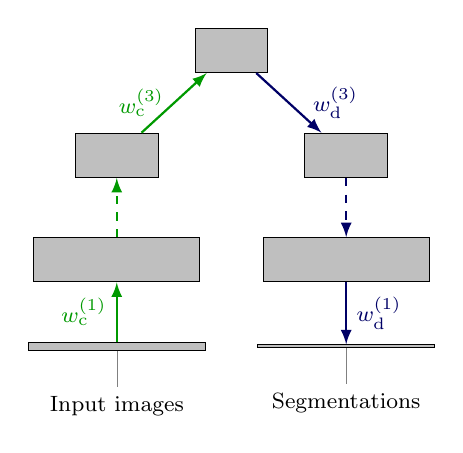
\begin{tikzpicture}[
  node distance=0.75cm and 0.65cm,
  font=\footnotesize,
  conv/.style={green!60!black,-latex,thick},
  conv2/.style={green!60!black,latex-latex,thick},
  deconv/.style={-latex,blue!40!black,thick},
  pooling/.style={-latex,green!60!black,thick,dashed},
  unpooling/.style={-latex,blue!40!black,thick,dashed},
  channel/.style args={#1 and #2}{draw, fill=lightgray, inner sep=0pt,
      minimum width=#1, minimum height=#2}
]

% Network

\node[channel=64pt and 3pt,pin=270:Input images] (inputs) {};
\node[channel=60pt and 16pt,above=of inputs] (clayer1) {};
\node[channel=30pt and 16pt,above=of clayer1] (pooling1) {};

\node[channel=64pt and 1pt,right=of inputs,pin=270:Segmentations] (outputs) {};
\node[channel=60pt and 16pt] (dlayer1) at (clayer1-|outputs) {};
\node[channel=30pt and 16pt,above=of dlayer1] (dpooling1) {};
\node[fit=(pooling1)(dpooling1),inner sep = 0pt] (pooling) {};
\node[channel=26pt and 16pt,above=of pooling] (clayer2) {};

\draw[conv] (inputs)--node[left] {$w^{(1)}_\text{c}$} (clayer1);
\draw[pooling] (clayer1)--node[left] {} (pooling1);
\draw[conv] (pooling1)--node[left] {$w^{(3)}_\text{c}$} (clayer2);
\draw[deconv] (clayer2)--node[right=5pt] {$w^{(3)}_\text{d}$} (dpooling1);
\draw[unpooling] (dpooling1)--node[right] {} (dlayer1);
\draw[deconv] (dlayer1)--node[right] {$w^{(1)}_\text{d}$} (outputs);
% \draw[deconv] (clayer1)--node[anchor=188,inner sep=10pt]
% {$w^{(1)}_\text{s}$}(outputs);

\end{tikzpicture}
\end{column}
\begin{column}{0.55\textwidth}
\centering
\begin{tikzpicture}
\node[inner sep=0pt] (image) {
  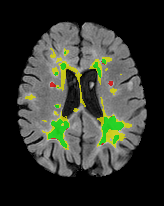
\includegraphics[width=0.45\textwidth]{images/p50s35_large_lesions_b}
};
\draw[white,thick] (-11pt,-14pt) circle (8pt);
\draw[white,thick] (13pt,-14pt) circle (9pt);

\end{tikzpicture}%
\hspace{4pt}%
\begin{tikzpicture}
[spy using outlines={circle, magnification=4, connect spies}]

\node[inner sep=0pt] (image) {
  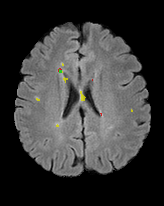
\includegraphics[width=0.45\textwidth]{images/p25s35_small_lesions_b}
};
\spy[white,thick, size=24pt,magnification=8] on (-9pt,18pt) in node[overlay]
at (-20pt,44pt);
\spy[white,thick, size=40pt] on (0pt,3pt) in node[overlay] at (24pt, 44pt);
\spy[white,thick, size=24pt, magnification=6] on (-11.5pt,-10.5pt) in
node[overlay] at (10pt,-46pt);

\node[below=1.5em of image,overlay,font=\footnotesize,align=right] {%
\textcolor{green!80!black}{Detected lesions}\\
\textcolor{yellow!80!black}{Missed lesions}\\
\textcolor{red!80!black}{False positives}};
\end{tikzpicture}
\end{column}
\end{columns}
\end{frame}

\begin{frame}[fragile]{Network Architecture: 7-layer CEN with shortcut}
\begin{columns}
\begin{column}{0.45\textwidth}
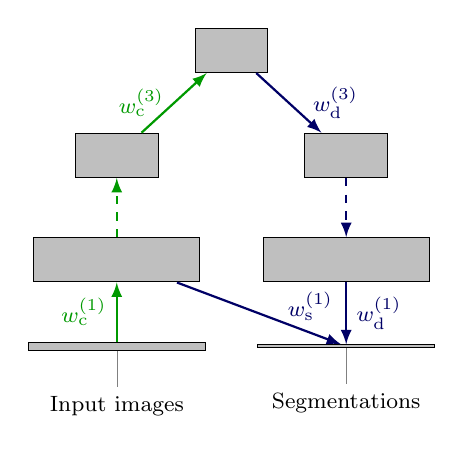
\begin{tikzpicture}[
  node distance=0.75cm and 0.65cm,
  font=\footnotesize,
  conv/.style={green!60!black,-latex,thick},
  conv2/.style={green!60!black,latex-latex,thick},
  deconv/.style={-latex,blue!40!black,thick},
  pooling/.style={-latex,green!60!black,thick,dashed},
  unpooling/.style={-latex,blue!40!black,thick,dashed},
  channel/.style args={#1 and #2}{draw, fill=lightgray, inner sep=0pt,
      minimum width=#1, minimum height=#2}
]

% Network

\node[channel=64pt and 3pt,pin=270:Input images] (inputs) {};
\node[channel=60pt and 16pt,above=of inputs] (clayer1) {};
\node[channel=30pt and 16pt,above=of clayer1] (pooling1) {};

\node[channel=64pt and 1pt,right=of inputs,pin=270:Segmentations] (outputs) {};
\node[channel=60pt and 16pt] (dlayer1) at (clayer1-|outputs) {};
\node[channel=30pt and 16pt,above=of dlayer1] (dpooling1) {};
\node[fit=(pooling1)(dpooling1),inner sep = 0pt] (pooling) {};
\node[channel=26pt and 16pt,above=of pooling] (clayer2) {};

\draw[conv] (inputs)--node[left] {$w^{(1)}_\text{c}$} (clayer1);
\draw[pooling] (clayer1)--node[left] {} (pooling1);
\draw[conv] (pooling1)--node[left] {$w^{(3)}_\text{c}$} (clayer2);
\draw[deconv] (clayer2)--node[right=5pt] {$w^{(3)}_\text{d}$} (dpooling1);
\draw[unpooling] (dpooling1)--node[right] {} (dlayer1);
\draw[deconv] (dlayer1)--node[right] {$w^{(1)}_\text{d}$} (outputs);
\draw[deconv] (clayer1)--node[anchor=188,inner sep=10pt]
{$w^{(1)}_\text{s}$}(outputs);

\end{tikzpicture}
\end{column}
\begin{column}{0.55\textwidth}
\centering
\begin{tikzpicture}
\node[inner sep=0pt] (image) {
  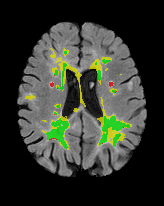
\includegraphics[width=0.45\textwidth]{images/p50s35_large_lesions_c}
};
\draw[white,thick] (-11pt,-14pt) circle (8pt);
\draw[white,thick] (13pt,-14pt) circle (9pt);

\end{tikzpicture}%
\hspace{4pt}%
\begin{tikzpicture}
[spy using outlines={circle, magnification=4, connect spies}]

\node[inner sep=0pt] (image) {
  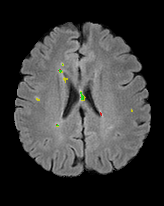
\includegraphics[width=0.45\textwidth]{images/p25s35_small_lesions_c}
};
\spy[white,thick, size=24pt,magnification=8] on (-9pt,18pt) in node[overlay]
at (-20pt,44pt);
\spy[white,thick, size=40pt] on (0pt,3pt) in node[overlay] at (24pt, 44pt);
\spy[white,thick, size=24pt, magnification=6] on (-11.5pt,-10.5pt) in
node[overlay] at (10pt,-46pt);

\node[below=1.5em of image,overlay,font=\footnotesize,align=right] {%
\textcolor{green!80!black}{Detected lesions}\\
\textcolor{yellow!80!black}{Missed lesions}\\
\textcolor{red!80!black}{False positives}};

\end{tikzpicture}
\end{column}
\end{columns}
\end{frame}

\section{Evaluation}

\subsection{Overview}

% TODO: Trained on different input modalities
% TODO: Explain what the measures are, what means good, how to interpret the
%       results
% TODO: Show quantitative results of good cases

\begin{frame}{Overview}
Evaluated on two data sets:
\begin{itemize}
\item MICCAI 2008 MS Lesion Segmentation Challenge
\begin{itemize}
\item 20 training, 23 testing images
\item Modalities: T1w, T2w, FLAIR 
\end{itemize}
\item Clinical trial data set
\begin{itemize}
\item 250 training, 77 testing images
\item Modalities: T1w, T2w, PDw, FLAIR
\item Compraed to 5 freely available methods
\item Stratified by average lesion size
\end{itemize}
\end{itemize}
\vspace{1em}
Evaluation measures:
\begin{itemize}
\item Dice similarity coefficient (DSC)
\item Lesion true positive rate (LTPR)
\item Lesion false positive rate (LFPR)
\item Volume difference (VD)
\end{itemize}
\end{frame}

\subsection{MICCAI 2008 Lesion Segmentation Challenge}

\begin{frame}{MICCAI 2008 Lesion Segmentation Challenge}
\sisetup{
  round-mode = places,
  round-precision = 2,
  detect-weight=true}%
Selected methods out of the 52 entries submitted for evaluation to the
MICCAI 2008 MS lesion segmentation challenge.
\begin{center}
\begin{tabular}{@{}clS[table-format=2.2]
S[table-format=2.1,round-precision=1]
S[table-format=2.1,round-precision=1]
S[table-format=2.1,round-precision=1]@{}}
\toprule
Rank & Method & {Score} & {LTPR} & {LFPR} & {VD} \\
\midrule
$1,3,9$  & Jesson et al. & 86.9386 & 48.70 & 28.25 & 80.15 \\
2  & Guizard et al.  & 86.1071 & 49.85 & 42.75 & 48.80 \\
$4,20,26$  & Tomas-Fernandez et. al & 84.464 & 46.9 & 44.6 &
45.60 \\
$5,7$ & Jerman et al.    & 84.1555 & 65.15 & 63.75 & 77.45 \\
\bfseries 6  & \bfseries Our method  & \bfseries 84.0743 & \bfseries 51.55 &
\bfseries 51.25 & \bfseries 57.75 \\
11 & Roura et al.   & 82.3442 & 50.15 & 41.85 & 111.60 \\
13 & Geremia et al.& 82.0691 & 55.1 & 74.1 & 48.90 \\
24 & Shiee et al. & 79.8975 & 52.4 & 72.7 & 74.45 \\
33 & Sudre et al. & 77.9601 & 22.3 & 18.1 & 285.6 \\
\bottomrule
\end{tabular}
\end{center}
\end{frame}

\subsection{Clinical Trial Data Set}

\begin{frame}{Clinical Trial Data Set}
\vspace{2em}
\begin{center}
\tikz[overlay] \node{%
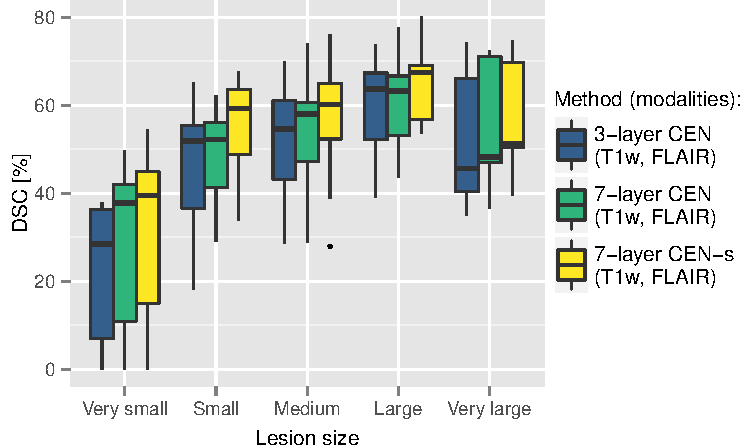
\includegraphics[width=\textwidth]{images/dsc_arch}};
\end{center}
\end{frame}

\begin{frame}{Clinical Trial Data Set}
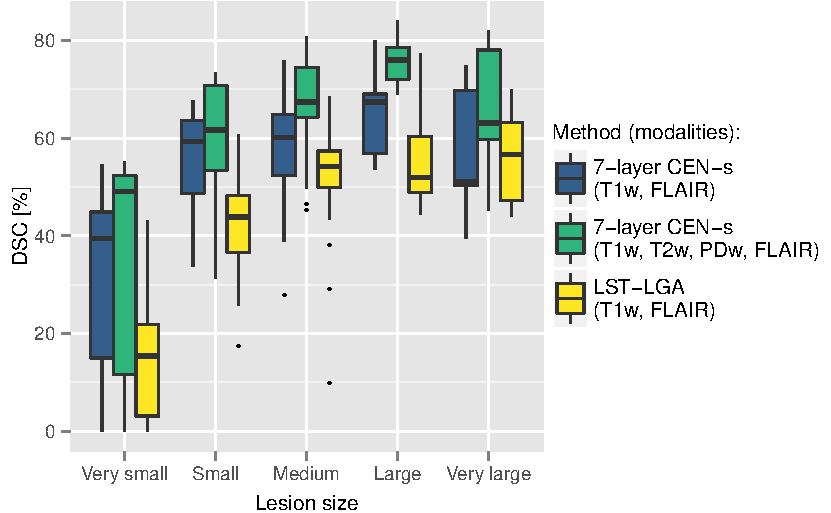
\includegraphics[width=1.02\textwidth]{images/dsc2}
\end{frame}

\begin{frame}{Clinical Trial Data Set}
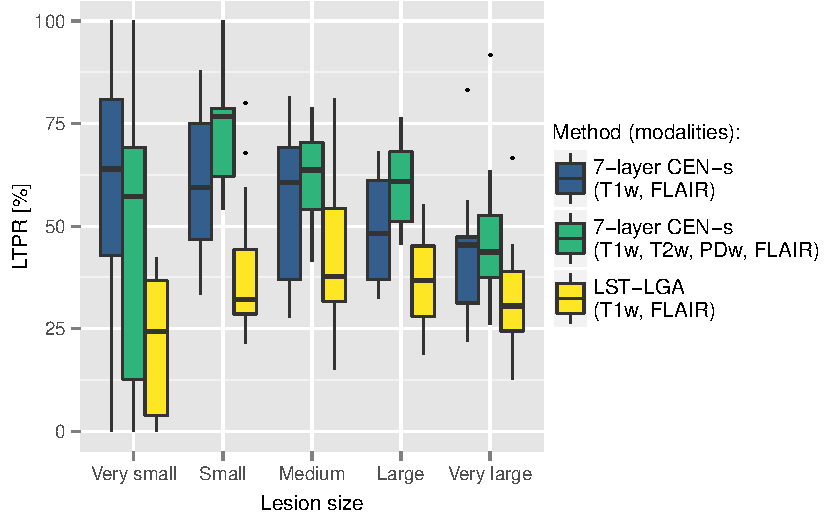
\includegraphics[width=1.02\textwidth]{images/tpr}
\end{frame}

\begin{frame}{Clinical Trial Data Set}
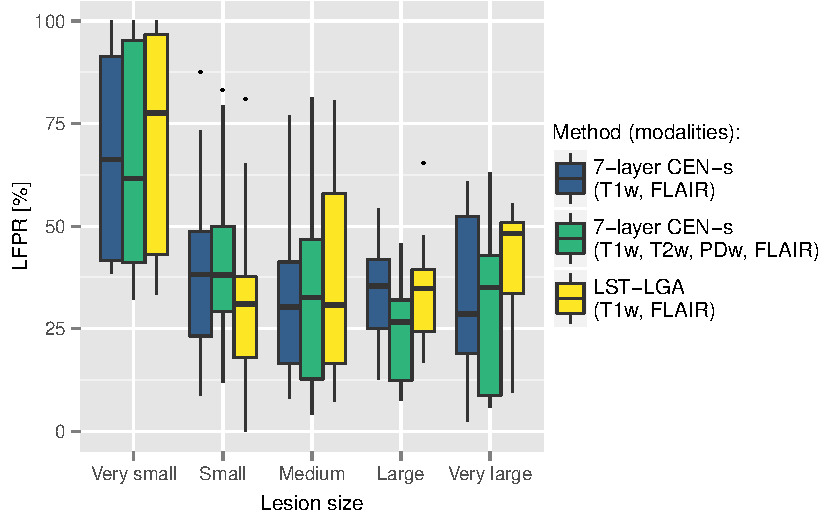
\includegraphics[width=1.02\textwidth]{images/fpr}
\end{frame}

\section{Conclusions}

\subsection{Summary}

\begin{frame}{Summary}
\begin{itemize}
\item Presented a segmentation method based on convolutional encoder networks
\item Joint learning of feature extractor and classifier facilitates the
learning that are tuned to a given combination of image modalities and
segmentation task
\item General framework $\Rightarrow$ can be applied to other segmentation
problems
\end{itemize}

\begin{itemize}
\item[\faQuestionCircle] What other structures are of interest?
\item[\faQuestionCircle] Do we have data to train the model? 
\end{itemize}
\end{frame}

\subsection{Future Work}

\begin{frame}{Future Work}
\begin{itemize}
\item Segmentation of the corpus callosum
\item<3-> Segmentation of the spinal cord
\item<5-> Segmentation of spinal cord grey matter
\end{itemize}
\begin{center}
\only<1>{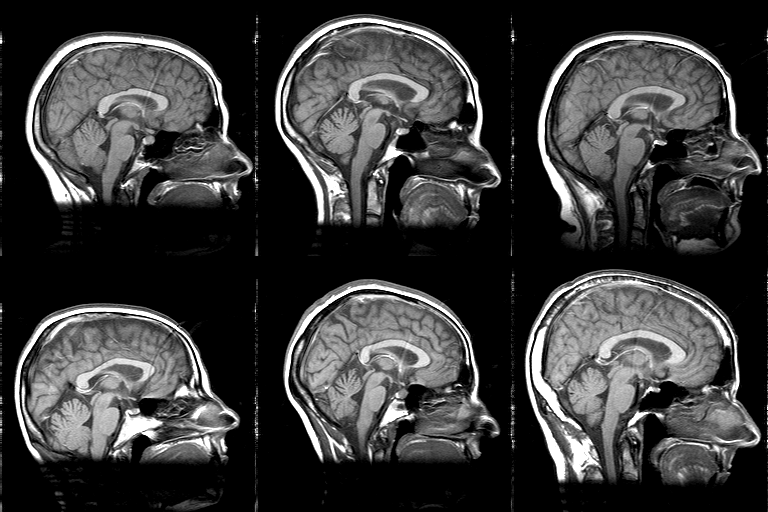
\includegraphics[height=0.45\textwidth]{images/T1w_6}}%
\only<2>{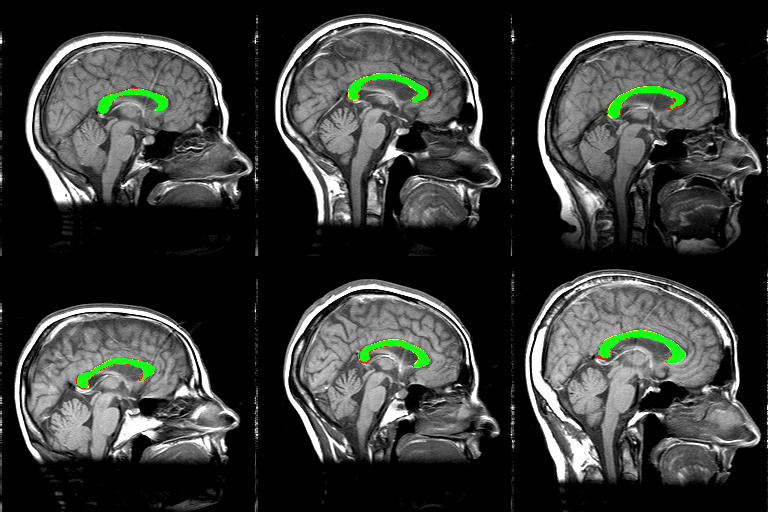
\includegraphics[height=0.45\textwidth]{images/segmentation_6}}%
\only<3>{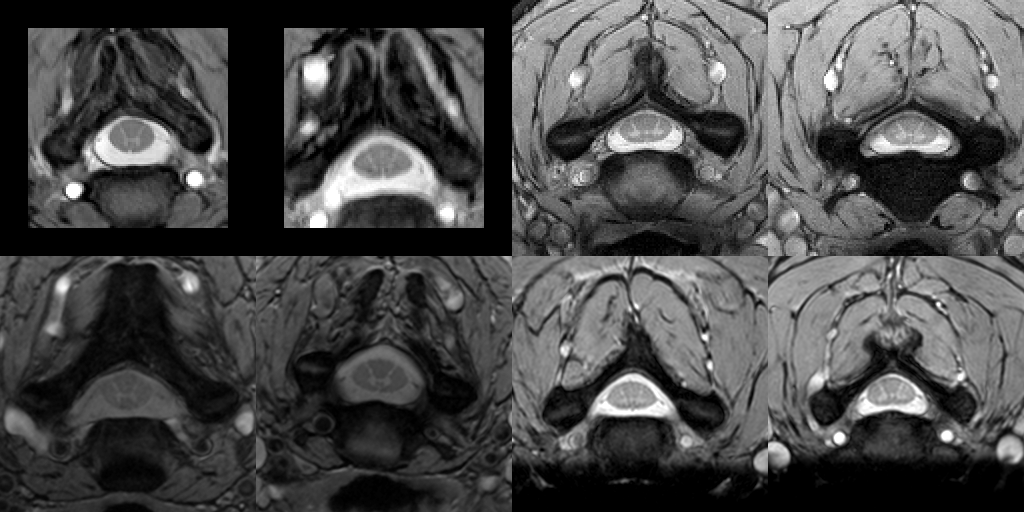
\includegraphics[height=0.45\textwidth]{images/T1w_8}}%
\only<4>{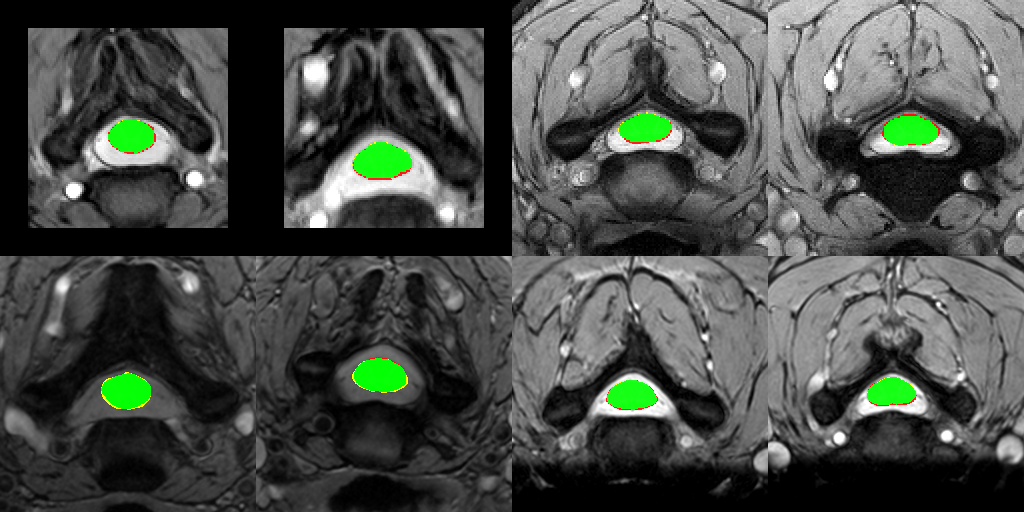
\includegraphics[height=0.45\textwidth]{images/WM_8}}%
\only<5>{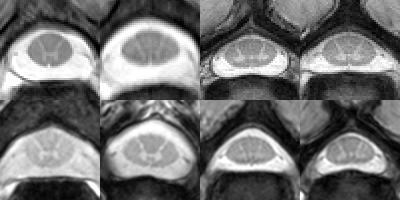
\includegraphics[height=0.45\textwidth]{images/T1w_roi_8}}%
\only<6>{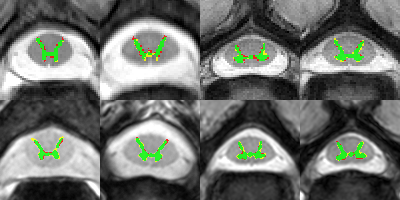
\includegraphics[height=0.45\textwidth]{images/GM_roi_8}}%
\end{center}
\end{frame}

\begin{questionmarks}
\begin{frame}
\centering
\Large Thank you for your attention.
\end{frame}
\end{questionmarks}

\appendix

\begin{frame}{Clinical Trial Data Set}
\begin{center}
\begin{tabular}{@{}lcccc@{}}
\toprule
Method & DSC [\%] & LTPR [\%] & LFPR [\%] & VD [\%] \\
\midrule
\multicolumn{5}{c}{\textit{Input modalities: T1w and FLAIR}} \\
\midrule
3-layer CEN & 49.24 & \bfseries 57.33 & 61.39 & 43.45 \\
7-layer CEN & 52.07 & 43.88 & \bfseries 29.06 & 37.01 \\ 
7-layer CEN-s & \bfseries 55.76 & 54.55 & 38.64 & 36.30 \\[0.2em]
Lesion-TOADS & 40.04 & 56.56 & 82.90 & 49.36 \\ 
SLS & 43.20 &  56.80 & 50.80 & \bfseries 12.30 \\
LST-LGA & 46.64 & 37.50 & 38.06 & 36.77 \\
LST-LPA & 46.07 & 48.02 & 52.94 & 41.62 \\
\bottomrule
\end{tabular}
\end{center}
\end{frame}

\begin{frame}{Clinical Trial Data Set}
\begin{center}
\begin{tabular}{@{}lcccc@{}}
\toprule
Method & DSC [\%] & LTPR [\%] & LFPR [\%] & VD [\%] \\
\midrule
\multicolumn{5}{c}{\textit{Input modalities: T1w and FLAIR}} \\
\midrule
7-layer CEN-s & 55.76 & 54.55 & 38.64 & 36.30 \\[0.2em]
Lesion-TOADS & 40.04 & 56.56 & 82.90 & 49.36 \\ 
LST-LGA & 46.64 & 37.50 & 38.06 & 36.77 \\
\midrule
\multicolumn{5}{c}{\textit{Input modalities: T1w, T2w, and PDw}} \\
\midrule
7-layer CEN-s & 61.18 & 52.00 & 36.68 & \bfseries 29.38 \\
EMS & 42.94 & 44.80 & 76.58 & 49.29 \\
\midrule
\multicolumn{5}{c}{\textit{Input modalities: T1w, T2w, FLAIR, and PDw}} \\
\midrule
7-layer CEN-s & \bfseries 63.83 & \bfseries 62.49 & \bfseries 36.10 & 32.89 \\
EMS & 39.70 & 49.08 & 85.01 & 34.51 \\
\bottomrule
\end{tabular}
\end{center}
\end{frame}

\begin{frame}{Stratified by Lesion Size}
Lesion size groups as used for the detailed analysis:

\begin{center}
\small
\begin{tabular}{@{}lccc@{}}
\toprule
Group & Mean lesion size [\si{\cubic\milli\metre}] & \#Samples & Lesion
load [\si{\cubic\milli\metre}] \\
\midrule
% 0, 1250, 2500, 3800, 10000
Very small & $[0,70]$ & 6 & \num{1457+-1492} \\
Small      & $(70,140]$ & 24 & \num{4298+-2683} \\
Medium & $(140,280]$ & 24 & \num{12620+-9991} \\
Large & $(280,500]$ & 14 & \num{13872+-5814} \\
Very large & $> 500$ & 9 & \num{35238+-27531} \\
\bottomrule
\end{tabular}
\end{center}
\end{frame}

\end{document}
